\documentclass[11pt]{article}

% Self-contained: compiles on Overleaf or any standard TeX install with no extra class files.
\usepackage[utf8]{inputenc}
\usepackage[T1]{fontenc}
\usepackage{amsmath,amssymb}
\usepackage{microtype}
\usepackage[margin=1in]{geometry}
\usepackage{hyperref}
\hypersetup{colorlinks=true,linkcolor=blue,citecolor=blue,urlcolor=blue}
\usepackage{xcolor}
\usepackage{listings}
\usepackage{tikz}
\usetikzlibrary{arrows.meta,positioning,fit,backgrounds}
\lstset{basicstyle=\ttfamily\small,breaklines=true,columns=fullflexible,frame=single,
        framesep=4pt,xleftmargin=4pt}

\newcommand{\Q}{Q}
\newcommand{\code}[1]{\texttt{#1}}

\title{The SMT Tractability Cliff in ML-DSA Modular-Arithmetic Verification:\\
       A Cross-Frontend Study over C and Rust}

\author{Amar Akshat\\Independent Researcher\\\texttt{amar.akshat@gmail.com}}
\date{\today}

\begin{document}
\maketitle

\begin{abstract}
Machine-checked equivalence between a cryptographic implementation and its specification is only
useful if the proof actually discharges. For the modular arithmetic at the core of ML-DSA
(FIPS~204)~\cite{fips204} we find that whether it discharges depends steeply, and measurably, on the
input domain --- and we map where the boundary lies, why it is there, and how to cross it. We study
reduction primitives and the forward number-theoretic transform (NTT) of two independent ML-DSA
implementations --- a reference and a library: the PQClean / pq-crystals C reference, via SAW, Cryptol,
and Isabelle/HOL composed
through the \code{cryptol-to-isabelle} translator into a single chain from C to a FIPS-derived
specification; and the RustCrypto implementation, via SAW over MIR. On the C side we obtain end-to-end
correctness for the \code{reduce.c} layer (\code{montgomery\_reduce}, \code{reduce32}, \code{caddq},
\code{freeze}) and a machine-checked overflow-freedom bound for the forward-NTT model. On the Rust side
we obtain SAW-verified equivalence for Barrett reduction, constant-time division, the twiddle-factor
table, and the hint layer (Algorithms 36, 37, 39, 40); the C NTT result is a machine-checked
overflow-freedom bound for the model, extended to the C by an argued composition. Against these positive
results we report the boundary: narrow-domain reductions discharge in seconds, while wide-domain Barrett
reduction over the full product domain $x < 2^{46}$ fails to complete across six solver and tactic
configurations, and a single NTT layer fails likewise. We isolate the structural cause: the \emph{same}
goal that times out as a bit-vector formula over $x<2^{46}$ discharges in $0.04$\,s when reformulated in
unbounded-integer arithmetic, identifying the bit-blasting of $(x \cdot M) \gg k$ --- not the modulus or
formula size --- as the wall, across the eager bit-blasting back-ends we tested. We give three proof
restructurings that target it. One we carry to completion: a total-coefficient-invariant induction that
replaces a $\sim$3000-obligation SAW unrolling with an eight-step proof running in seconds. For a second,
an unbounded-integer reformulation, we show the integer core discharges and only the bitvector bridge
remains; a third, a compositional specification, we identify. We also report
two off-by-one defects in the reference's documented contracts, disclosed upstream. The toolchain's
maintainers independently confirm both the boundary and the integer-reformulation escape. The development
uses no vendor verification artifacts; the main proof pipeline runs from a single command, and the
timeout and encoding experiments are reproduced by self-contained scripts.
\end{abstract}

\medskip
\noindent\textbf{Keywords:} ML-DSA $\cdot$ FIPS 204 $\cdot$ formal verification $\cdot$ SMT
$\cdot$ SAW $\cdot$ Cryptol $\cdot$ Isabelle/HOL $\cdot$ MIR $\cdot$ Barrett reduction $\cdot$
number-theoretic transform $\cdot$ tractability.

\section{Introduction}\label{sec:intro}

ML-DSA (FIPS~204)~\cite{fips204} is the NIST-standardized lattice signature scheme derived from
CRYSTALS-Dilithium~\cite{dilithium}. Its security analysis assumes that implementations compute the
specified function. Test vectors check that assumption on a finite set of inputs; formal verification
checks it for all inputs, which matters for arithmetic kernels whose bugs are input-dependent and can
pass test vectors~\cite{eprint1032}.

A practitioner who sets out to machine-check these kernels against the specification quickly meets a
less-discussed obstacle: many of the proofs do not discharge. The same SAW/SMT formulation that proves
one reduction in seconds runs for hours, or never finishes, on another that differs only in its input
range. This is folklore among verification engineers, but it is rarely characterized: \emph{where} the
boundary sits, \emph{why}, and \emph{what to do instead} are usually left implicit.

This paper maps that boundary for ML-DSA's modular arithmetic, concretely and reproducibly, across two
independent implementations and two verification toolchains. We treat the cases that do not discharge not
as failures to hide but as the primary result: a characterized tractability boundary, its structural
cause, and the proof restructurings that cross it. The positive verification results --- a complete
reduction layer and an overflow-freedom bound on the C side, and a verified field, division,
twiddle-table, and hint layer on the Rust side --- establish what sits on the tractable side of the
boundary and anchor the study.

\paragraph{Contributions.}
\begin{enumerate}
  \item \textbf{A reproducible tractability map} for SMT-based equivalence verification of PQC modular
  arithmetic (Section~\ref{sec:boundary}). We characterize, with timings, which arithmetic-kernel
  equivalences discharge automatically and which do not: narrow-domain Barrett reduction ($x < 2^{28}$)
  proves in about four seconds, while the same goal over the cryptographically relevant wide domain
  ($x < 2^{46}$) does not complete under \code{z3}, \code{abc}, \code{cvc5}, \code{yices}, a
  \code{goal\_eval} rewrite pass, or a carry-fold reformulation.
  \item \textbf{The structural cause, isolated.} The wall is the bit-vector formula for $(x \cdot M) \gg k$
  --- a constant multiply and a power-of-two shift related to $x \bmod Q$ --- which failed to discharge
  under every solver and tactic configuration we tried, with solve time growing steeply in the live input
  width. We isolate bit-blasting as the cause with a controlled experiment: the same goal over $x<2^{46}$,
  reformulated in unbounded-integer arithmetic, discharges in $0.04$\,s where the bit-vector form times
  out (Section~\ref{sec:boundary}). The same shape recurs in Barrett reduction and, 256-fold, in one NTT
  layer. The evidence locates the difficulty in the goal shape across the eager bit-blasting back-ends
  tested, not in one back-end; we do not claim a solver-independent impossibility result.
  \item \textbf{One completed escape, and two identified.} A total-coefficient invariant turns an
  intractable $\sim$3000-obligation SAW unrolling of NTT overflow-freedom into an eight-step Isabelle
  induction running in seconds (Section~\ref{sec:ntt}); this escape we carry to completion. For a second
  --- an unbounded-integer reformulation with a bitvector bridge for the reductions --- we demonstrate
  that the integer core discharges in $0.04$\,s, leaving only the bridge; a third, a compositional
  specification for the layer proof, we identify (Section~\ref{sec:boundary}).
  \item \textbf{A cross-frontend, cross-language study.} The same primitives are verified in two
  pipelines --- LLVM+Cryptol+Isabelle on the C reference (Section~\ref{sec:reduce}) and MIR+Cryptol on
  the RustCrypto implementation (Section~\ref{sec:rust}). Both share SAW as the symbolic-execution engine;
  the independence is in the language frontend (LLVM vs.\ MIR) and, on the C side, an added
  Isabelle proof-obligation backend. Reproducing the same tractability symptom across two frontends and
  two languages is evidence that the boundary is induced primarily by the goal shape rather than by a
  single frontend.
  \item \textbf{Two off-by-one defects} in the reference's documentation contracts, reproduced against
  the shipping code and disclosed upstream to pq-crystals/dilithium (Section~\ref{sec:findings}).
\end{enumerate}

\paragraph{Non-claims.} We verify reference and library implementations, not the optimized
AVX2/aarch64 paths or the \code{mldsa-native} successor, where the most error-prone arithmetic lives. We
prove C/Rust $\equiv$ model and overflow-freedom; we do not prove NTT \emph{transform} correctness, that
is, equivalence of the model to the negacyclic transform of FIPS~204 Algorithms 41 and 42. The
wide-domain reductions and the NTT-layer transform proof are reported as a characterized boundary with
escapes identified, \emph{not} as completed proofs. We say nothing about constant-time behavior.

\paragraph{Status of each claim.} Because the value of a verification paper is in the precise status of
each claim, we summarize them up front (Table~\ref{tab:status}); ``mechanized'' means a tool discharged
the goal in this development with no \code{sorry}, \code{oops}, or admitted goal.

\begin{table}[h]
\centering\small
\begin{tabular}{lll}
\hline
Claim & Status & Trust base \\
\hline
\code{reduce.c}: C $\equiv$ Cryptol & mechanized (SAW) & LLVM, SAW, Cryptol \\
\code{reduce.c}: model $\equiv$ spec & mechanized (Isabelle) & no \code{sorry}/\code{oops} \\
C NTT: C $\equiv$ model (\code{-fwrapv}) & mechanized (SAW) & \code{montgomery\_reduce} override \\
C NTT: overflow-freedom & mechanized for model; C bridge argued & Isabelle + composition \\
Rust Barrett / division / table / hint & mechanized (SAW over MIR) & \code{mir-json}, 3 leaf assumptions \\
Wide-domain Barrett ($x<2^{46}$), bit-vector & not proven --- timeout study & empirical boundary \\
Wide-domain Barrett, integer core & discharged (z3, NIA, $0.04$\,s) & escape-2 core; bridge open \\
NTT transform $\equiv$ FIPS Alg.\ 41/42 & not attempted to completion & --- \\
\hline
\end{tabular}
\caption{Status of each result. ``Argued'' and ``empirical boundary'' rows are not mechanized theorems.}
\label{tab:status}
\end{table}

\section{Background}\label{sec:background}

\paragraph{Targets.} On the C side we verify PQClean~\cite{pqclean} \code{ml-dsa-44/clean}, files
\code{reduce.c} and \code{ntt.c}, pinned by commit hash; this code is byte-identical to
pq-crystals/dilithium~\cite{dilithium} up to a namespace prefix. (PQClean is scheduled for read-only
archival in July 2026; because the vendored target is byte-identical to the canonical
pq-crystals/dilithium reference, the results transfer to it and to the PQ Code Package
\code{mldsa-native} successor.) On the Rust side we verify
RustCrypto's \code{ml-dsa} crate~\cite{rustcrypto} and its shared \code{module-lattice} field core. ML-DSA
fixes the prime modulus $Q = 8380417$ and ring dimension $N = 256$. \code{montgomery\_reduce} maps a
64-bit input to a 32-bit value congruent to $a \cdot 2^{-32} \pmod Q$. \code{reduce32} is a
Barrett-style reduction to a centered window; RustCrypto instead uses an explicit Barrett reduction
$x \mapsto x - \lfloor (x \cdot M) / 2^{k} \rfloor\, Q$ with $M = \lfloor 2^{k}/Q \rfloor$. The forward
NTT applies eight levels of Cooley-Tukey butterflies, each multiplying a coefficient by a precomputed
twiddle factor and reducing.

\paragraph{Tools.} SAW (the Software Analysis Workbench)~\cite{saw} proves a compiled function
equivalent to a Cryptol specification by symbolic execution and SMT; it targets LLVM bitcode for C and,
via \code{mir-json}, Rust MIR. Cryptol is a word-level specification language. Isabelle/HOL is an
interactive theorem prover. The \code{cryptol-to-isabelle} translator, first shipped with saw-script
1.5.1, lifts a Cryptol module into an Isabelle theory; we use it to compose the two C-side proof legs.
All tool versions are pinned (Section~\ref{sec:repro}).

\section{The two pipelines}\label{sec:pipeline}

\begin{figure}[h]
\centering
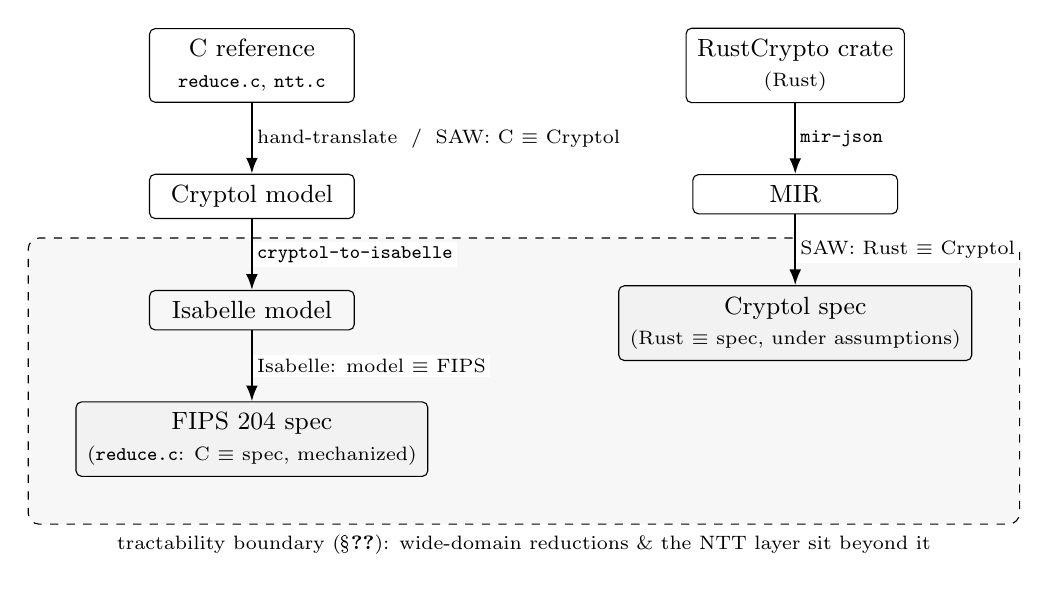
\begin{tikzpicture}[
  font=\small,
  node distance=9mm and 22mm,
  box/.style={draw, rounded corners=2pt, align=center, inner sep=4pt, minimum width=26mm},
  proven/.style={box, fill=black!5},
  flow/.style={-{Latex[length=2mm]}, thick},
  lbl/.style={font=\scriptsize, midway, fill=white, inner sep=1.5pt}
]
  % C pipeline (left column)
  \node[box] (cref) {C reference\\\scriptsize\code{reduce.c}, \code{ntt.c}};
  \node[box, below=of cref] (cmod) {Cryptol model};
  \node[box, below=of cmod] (imod) {Isabelle model};
  \node[proven, below=of imod] (cspec) {FIPS 204 spec\\\scriptsize(\code{reduce.c}: C $\equiv$ spec, mechanized)};
  \draw[flow] (cref) -- node[lbl, right] {hand-translate \;/\; SAW: C $\equiv$ Cryptol} (cmod);
  \draw[flow] (cmod) -- node[lbl, right] {\code{cryptol-to-isabelle}} (imod);
  \draw[flow] (imod) -- node[lbl, right] {Isabelle: model $\equiv$ FIPS} (cspec);

  % Rust pipeline (right column)
  \node[box, right=42mm of cref] (rcrate) {RustCrypto crate\\\scriptsize(Rust)};
  \node[box, below=of rcrate] (mir) {MIR};
  \node[proven, below=of mir] (rspec) {Cryptol spec\\\scriptsize(Rust $\equiv$ spec, under assumptions)};
  \draw[flow] (rcrate) -- node[lbl, right] {\code{mir-json}} (mir);
  \draw[flow] (mir) -- node[lbl, right] {SAW: Rust $\equiv$ Cryptol} (rspec);

  % boundary band
  \begin{scope}[on background layer]
    \node[draw, dashed, rounded corners, fill=black!3, fit=(cspec)(rspec),
          inner sep=6mm, label={[font=\scriptsize]below:tractability boundary (\S\ref{sec:boundary}): wide-domain reductions \& the NTT layer sit beyond it}] {};
  \end{scope}
\end{tikzpicture}
\caption{Two pipelines over the same primitives. The C pipeline composes a SAW leg (C $\equiv$ Cryptol)
and an Isabelle leg (model $\equiv$ FIPS), connected by \code{cryptol-to-isabelle}, into a single chain
from C to a FIPS-derived specification. The Rust pipeline verifies MIR directly against Cryptol with SAW.
Both reach the same tractability boundary (Section~\ref{sec:boundary}).}
\label{fig:pipeline}
\end{figure}

The C model is hand-translated at the exact bit widths, because the algorithms depend on two's-complement
truncation and signed shifts and SAW checks bit-for-bit equivalence. The lift step is mechanical: a
continuous-integration check (\code{make lift-check}) regenerates the Isabelle theory from the
\code{.cry} source and diffs it against the committed copy, so no human-maintained link sits between the
two legs. The Rust pipeline builds MIR with \code{mir-json}~\cite{mirjson} (pinned to the schema version
SAW~1.5.1 bundles) from a small harness crate that exercises keygen, sign, and verify so the generic
field and transform code monomorphizes; SAW then verifies the monomorphized functions against Cryptol.

\section{The \code{reduce.c} layer (C)}\label{sec:reduce}

\paragraph{C $\equiv$ Cryptol.} SAW discharges bit-exact equivalence for all four functions on the
default (overflow-checking) LLVM bitcode, so the proofs also assert absence of signed-overflow undefined
behavior on the relevant ranges. \code{montgomery\_reduce} is verified under its documented input range.
\code{reduce32} is verified under $a \le 2^{31} - 2^{22} - 1$, the bound that keeps the internal
\code{a + (1{<}{<}22)} addition from overflowing. \code{caddq} is verified unconditionally. \code{freeze}
is verified compositionally using the \code{reduce32} and \code{caddq} results as overrides. A mutation
test confirms the \code{montgomery\_reduce} proof is non-vacuous: a deliberately wrong model is rejected
with a counterexample.

\paragraph{Model $\equiv$ specification.} In Isabelle we state each function's contract and prove the
lifted model meets it, with no \code{sorry} or \code{oops}.
\begin{itemize}
  \item \code{montgomery\_reduce}: $2^{32} r \equiv a \pmod Q$ and $-Q < r < Q$ on the half-open domain
  $-2^{31} Q \le a < 2^{31} Q$.
  \item \code{caddq}: residue-preserving, and maps $[-Q, Q)$ into $[0, Q)$.
  \item \code{reduce32}: residue-preserving, with output in the window $[-6283009, 6283008]$ on
  $a \le 2^{31} - 2^{22} - 1$.
  \item \code{freeze}: residue-preserving, with output in $[0, Q)$, proven from the previous two.
\end{itemize}
Composing with the SAW leg gives a statement from C to specification: on the documented ranges, each
reference function computes a correct residue modulo $Q$ within its proven output window. The
windows above are the \emph{true reachable} windows, which differ from the documented ones for two
functions (Section~\ref{sec:findings}). This layer sits entirely on the tractable side of the boundary:
the inputs are single machine words and the goals discharge in seconds.

\section{The RustCrypto layer (Rust)}\label{sec:rust}

The RustCrypto pipeline reaches the same primitives in a different language and toolchain, and the same
narrow-domain goals discharge. All results below are SAW-verified against a Cryptol specification; the
reduction proofs additionally carry a mutation test in continuous integration --- a deliberately altered
modulus is rejected --- so they are not vacuously true.
\begin{itemize}
  \item \textbf{Barrett reduction} $== x \bmod m$ for all \code{u32} inputs, for each modulus
  $m \in \{Q = 8380417,\ 2\gamma_2 = 190464,\ 2^d = 8192\}$ that occurs, with the conditional final
  subtraction live; no precondition is needed because each modulus exceeds $2^{16}$. (Here $m$ is the
  reduction modulus, distinct from the Barrett multiplier $M = \lfloor 2^k/Q \rfloor$ of
  Section~\ref{sec:boundary}.)
  \item \textbf{Constant-time division} $\code{ct\_div}(x) == \lfloor x / 190464 \rfloor$ on its
  documented domain $x < Q$.
  \item \textbf{Twiddle-factor table}: every constant-folded copy of the 256-entry table equals
  $\zeta^{\mathrm{BitRev}_8(i)} \bmod Q$.
  \item \textbf{Hint layer}: \code{decompose}, \code{high\_bits}, \code{make\_hint}, and
  \code{use\_hint} equal FIPS~204 Algorithms 36, 37, 39, and 40 respectively, over all field elements.
\end{itemize}
Three leaf operations are constant-time intrinsics or inline assembly (a \code{black\_box} identity and
two conditional-move primitives); these are supplied as assumed specifications, each justified against
the target assembly, and recorded as the verification's trust base alongside \code{mir-json} soundness.

\section{Forward-NTT overflow-freedom, and the first escape}\label{sec:ntt}

The forward NTT performs unreduced \code{int32} additions and subtractions, $a[j] \pm t$, which overflow
for unbounded inputs. On a \code{-fwrapv} build, where signed overflow is two's-complement wrapping, SAW
proves the C NTT functionally equivalent to the Cryptol model for all inputs, with \code{montgomery\_reduce}
supplied as an uninterpreted override so the 1024 butterfly calls collapse to a structural array
equality. This proof says nothing about overflow.

Overflow-freedom is the property of interest, since it is the defect class behind known ML-DSA
implementation bugs that passed test vectors~\cite{eprint1032}. The statement \code{ntt\_overflow\_free}
is: if every input coefficient lies in $\pm(2^{31} - 2^{27})$, then every coefficient of the transform
lies in $\pm 2080309256 < 2^{31} - 1$. We prove it by induction over the eight levels. A single per-level
lemma states that one level grows the maximum coefficient magnitude by at most $Q$; the growth bound
comes from the \code{montgomery\_reduce} output bound $|t| < Q$. Iterated eight times from an input bound
with headroom $2^{27} > 8Q$, every intermediate value stays below $2^{31}$, so each \code{int32}
addition and subtraction has its true result in range and does not overflow.

\paragraph{The total invariant (escape one).} The enabling device is the form of the invariant. The
Cryptol index operation is strict, but an out-of-bounds access returns the last element of the sequence.
We therefore state the coefficient bound over \emph{all} indices, not only the valid ones. Every indexed
access is then a bounded list member, in-bounds or not, so the proof never reasons about the modular
index arithmetic of the butterfly network --- shifts and divisions parameterized by the level, the exact
arithmetic that made the direct SMT approach intractable (Section~\ref{sec:boundary}). This is the one
restructuring we carry to completion: a change of proof structure, not of solver, turns an intractable
goal tractable.

\paragraph{From the model to the C.} The Isabelle result is about the model. SAW proves the C equal to
the model for all inputs on the \code{-fwrapv} build; the Isabelle result shows the model does not wrap
under the input bound; the two builds differ only in whether signed overflow is poison. Hence we argue that the
reference C NTT has no signed-overflow undefined behavior under the bound. We state this composition
explicitly rather than mechanize it as one SAW theorem, because the direct attempt did not complete
(Section~\ref{sec:boundary}); it is an argued meta-step over two mechanized results, not itself a machine-checked theorem.

\section{The tractability boundary}\label{sec:boundary}

The reduction layer and the field, division, and hint layers above all discharge in seconds. The
transform layer does not, and the transition is steep, measurable, and reproducible.

\paragraph{Wide-domain Barrett.} RustCrypto's Barrett reduction computes, in \code{u128},
$\code{product} = x \cdot M$ with $M = \lfloor 2^{46}/Q \rfloor = 8396807$, $\code{quotient} =
\code{product} \gg 46$, $\code{remainder} = x - \code{quotient} \cdot Q$, then a conditional subtraction.
The field multiplication that feeds it produces $x = a \cdot b$ with $a, b < Q < 2^{23}$, so the relevant
input domain is $x < 2^{46}$. We verify $\code{barrett\_reduce}(x) == x \bmod Q$ against an increasing
input bound (z3, single thread, Apple M4, 16\,GB, 300\,s timeout):
\begin{center}
\begin{tabular}{ll}
\hline
input bound & wall-clock (z3) \\
\hline
$x < 2^{20}$ & 3.7\,s \\
$x < 2^{28}$ & 4.1\,s \\
$x < 2^{30}$ & 7.3\,s \\
$x < 2^{32}$ & 27.9\,s \\
$x < 2^{34}$ & 183.6\,s \\
$x < 2^{36}$ & $>300$\,s (no completion) \\
$x < 2^{44},\, 2^{46}$ & $>300$\,s (no completion) \\
\hline
\end{tabular}
\end{center}
Solve time is flat up to about $2^{28}$ and then grows by a factor of roughly four to seven per two
added bits ($7.3 \to 27.9 \to 183.6$\,s), crossing the timeout between $2^{34}$ and $2^{36}$ ---
consistent with exponential growth in the live input width, not in the modulus or the formula size,
though the growth region spans only three points. At $x < 2^{46}$ the goal also failed to
complete under \code{abc}, \code{cvc5}, \code{yices}, a \code{goal\_eval} rewrite pass before \code{z3},
and a hand-written carry-fold reformulation of the specification (six configurations in all, each to the
same 300\,s timeout). All five solver back-ends decide \code{QF\_BV} by eager bit-blasting (\code{z3},
\code{cvc5}, \code{yices} bit-blast; \code{abc} reasons on the AIG directly), so the experiment varies the
solver but not the bit-blasting strategy. The corresponding narrow-domain Barrett reduction over
\code{u32} inputs, used elsewhere in ML-DSA, proves in seconds (Section~\ref{sec:rust}); the difference is
the live input width alone.

\paragraph{The structural cause.} The decisive subterm is $(x \cdot M) \gg 46$: a product just above
$2^{69}$ (a 70-bit value, since $M > 2^{23}$) divided by a power of two and related back to $x \bmod Q$.
The bit-vector \emph{formula} is not
itself large --- $M$ is a constant, so the multiply and shift are polynomial in width --- but the SAT
instance the solver must decide grows with the number of live input bits. When the precondition pins $x$
to a narrow range the high-order bits of the product are forced to zero and the instance collapses; over
the full $2^{46}$ domain none of those bits are fixed, and the instance did not complete under any
back-end we tried.

\paragraph{Isolating bit-blasting (a controlled experiment).} To test that bit-blasting specifically ---
not the arithmetic relation itself --- is the wall, we re-pose the \emph{same} obligation in unbounded
integer arithmetic. We ask \code{z3} (logic \code{NIA}) whether
$x - \lfloor x M / 2^{46} \rfloor\,Q \in [0, 2Q)$ for all $x \in [0, 2^{46})$, encoded as the negation; an
\code{unsat} answer establishes the identity over the whole domain. It returns \code{unsat} in
$0.04$\,s. The bit-vector form of the identical goal does not complete (Table above; $>300$\,s). A
non-vacuity mutation --- replacing $Q$ by $Q+1$ --- flips the integer query to \code{sat} with an explicit
witness ($x = 16760835$), so the fast \code{unsat} is not a modeling artifact. Same relation, same domain,
two encodings, four orders of magnitude apart: the difficulty is the bit-blasting of $(x \cdot M) \gg k$,
not the modular relation. (This integer identity is also the core of escape two below; what remains there
is the bit-vector-to-integer bridge.) The three \code{.smt2} files and a runner are in the artifact.

The boundary thus tracks the goal encoding rather than one back-end: across the eager bit-blasting
strategies tested it appears where a wide-domain $(x \cdot M) \gg k$ must be related to $x \bmod Q$ at
bit-vector width, and it falls where the live input width stops collapsing the instance --- here between
$2^{34}$ and $2^{36}$. Two caveats bound the claim. We tested only eager bit-blasting; \code{bitwuzla},
whose CEGAR-style abstraction-refinement targets exactly wide-bitwidth multiplication, is outside our
pinned toolchain and may shift the bit-vector boundary --- we leave that evaluation open. And the integer
result shows the relation is not intrinsically hard. We therefore report an empirical tractability
boundary for the eager bit-vector encodings tested, not a solver-independent impossibility result.

\paragraph{The NTT layer, same cause $\times 256$.} The same shape recurs in the transform. We attempted
one forward NTT layer (\code{ntt\_layer} with $\mathrm{LEN}=128$) against a FIPS~204 Algorithm~41 layer
specification, with the four field operations supplied as assumed specifications via
\code{mir\_unsafe\_assume\_spec} so the butterfly reduces to specification-form arithmetic. The overrides
apply and symbolic simulation completes, but the final proof obligation does not discharge: the
specification computes $(\cdot) \bmod Q$ independently for each of 256 output coefficients ---
256 bit-vector remainder-by-constant operations --- and these do not term-match the implementation's
reduce-after-each-operation structure, so the solver bit-blasts all of them. This is the wide-modular
reduction wall again, multiplied across the array.

\paragraph{Escapes two and three.} The total-invariant induction of Section~\ref{sec:ntt} is the first
escape and the one we carried to completion. Two others are the route past the remaining walls.
(2) An \emph{unbounded-integer reformulation}: prove the Barrett identity
$x - ((x \cdot M)\gg k)\,Q \equiv x \pmod Q$ and $\in [0, 2Q)$ in unbounded-integer arithmetic, then
bridge bit-vector to integer --- the structure by which we proved \code{montgomery\_reduce} on the C side.
The integer core of this escape is the controlled experiment above: it discharges in $0.04$\,s where the
bit-vector form times out, so what remains is mechanizing the bit-vector-to-integer bridge in SAW or
Isabelle, not the arithmetic. (3) A \emph{compositional specification}: build the layer specification from
the same override terms the implementation uses, so the two sides are syntactically the same term and the
obligation discharges by rewriting rather than bit-blasting 256 independent remainders; this one we
identify but have not yet realized. The maintainers of SAW endorse this route --- the same
\code{mir\_unsafe\_assume\_spec}-to-\code{Integer} plus goal-rewriting technique they applied to
Montgomery reduction~\cite{saw3306}; mechanizing the transform layer through these escapes is the
immediate next step.

\section{Findings}\label{sec:findings}

Establishing the true output windows in Section~\ref{sec:reduce} surfaced two off-by-one errors in the
reference's documentation comments. Both are documentation-contract defects, not miscomputations: the
functions return correct residues, but the stated bounds are wrong at boundary inputs that real call
sites do not reach. Both were verified against the shipping C.

\paragraph{OF-1.} The \code{montgomery\_reduce} comment states $-Q < r < Q$ (strict) over the inclusive
domain $-2^{31} Q \le a \le Q \cdot 2^{31}$. At $a = 2^{31} Q$ the function returns $r = Q$, violating the
strict upper bound. The guarantee that holds over the inclusive domain is $-Q \le r \le Q$; the strict
bound holds on the half-open domain, which is what we specify.

\paragraph{OF-2.} The \code{reduce32} comment states $-6283008 \le r \le 6283008$ for $a \le 2^{31} -
2^{22} - 1$. That precondition is one-sided, so $a = -2143289344$ is admissible and returns $r =
-6283009$, one below the stated bound. The stated bound holds only under the symmetric precondition
$|a| \le 2^{31} - 2^{22} - 1$.

Both comments are identical in \code{pq-crystals/dilithium} (the origin; PQClean re-namespaces it), so
the finding was reported there as a single issue. We did not file automatically; disclosure was
deliberate.

\section{Scope and limitations}\label{sec:scope}

The verified code is reference C and a Rust library, not the deployed AVX2/aarch64 or the
\code{mldsa-native} successor, where the genuinely error-prone optimized arithmetic lives. We prove
C/Rust $\equiv$ model and, for the C NTT, overflow-freedom; we do not prove NTT \emph{transform}
correctness against FIPS~204 Algorithms 41 and 42. The wide-domain Barrett reduction and the NTT-layer
transform proof are reported as a characterized boundary with one completed escape, one whose integer core
is demonstrated, and one identified --- not as completed proofs; the C-side overflow-freedom statement is
the composition argued in Section~\ref{sec:ntt}, not a single mechanized theorem. The Rust verification rests on \code{mir-json} soundness and the three assumed
constant-time leaf specifications of Section~\ref{sec:rust}. We say nothing about constant-time behavior.

\section{Reproducibility}\label{sec:repro}

The development is public and all tool versions are pinned by setup scripts: SAW 1.5.1 with its bundled
Cryptol and \code{cryptol-to-isabelle}, Isabelle2025-2 with a pinned AFP snapshot, a fixed clang, and for
the Rust pipeline a pinned Rust nightly with \code{mir-json} at the schema commit SAW 1.5.1 bundles. The
target C is vendored with its commit hash; the Rust crate is vendored likewise. A single command,
\code{make verify}, runs the lift check, the SAW leg, and the Isabelle leg; the Rust proofs run from the
same toolchain. Continuous integration runs the fast SAW gates on every push and the full pipeline on
demand. The wide-domain Barrett timeout map and the integer-versus-bit-vector contrast of
Section~\ref{sec:boundary} are reproduced by self-contained scripts in the repository (the latter ships
the three \code{.smt2} files and a runner). The exact pinned versions are:

\begin{lstlisting}
SAW                 1.5.1 (release v1.5.1, 1f227d9)
Cryptol             3.5.0 (bundled with SAW 1.5.1)
cryptol-to-isabelle bundled with saw-script 1.5.1
Isabelle            Isabelle2025-2
AFP snapshot        afp-2026-06-05
clang               Apple clang 17.0.0 (clang-1700.0.13.5)
rustc               nightly-2025-09-14 (1.91.0-nightly 02c7b1a7a)
mir-json            7e12cece (schema v8 = SAW 1.5.1 bundle)
SMT/SAT back-ends   z3 4.8.14, cvc5 1.3.1, yices 2.6.5, abc 1.01
host (timings)      Apple M4, 16 GB, macOS (arm64)
timeout             300 s wall-clock, single thread
\end{lstlisting}

\noindent The artifact is archived on Zenodo, DOI
\href{https://doi.org/10.5281/zenodo.20641411}{10.5281/zenodo.20641411}, and the source is at
\url{https://github.com/amarshat/pqc-assay}.

\section{Related work}\label{sec:related}

Apple's 2026 corecrypto verification~\cite{corecrypto} covers ML-KEM and ML-DSA in production code with
SAW, Cryptol, and Isabelle, proving the Cryptol models faithful to FIPS~203/204, and is the direct
methodological precedent for the C pipeline. Their pipeline discharges the wide-arithmetic goals through
the interactive Isabelle leg --- structured proof rather than automated SMT over the wide bit-vector
goal --- which is consistent with, not a counterexample to, our finding: the boundary is not that the
relation cannot be proven, but that it does not fall to eager bit-blasting, so a verifier must restructure
(as Apple does, and as our completed escape and the integer reformulation do). We do not claim a result
beyond Apple's; we apply the same public toolchain independently to reference C, add a second frontend
over Rust MIR, and center the tractability boundary and its escapes rather than a single implementation.
The PQ Code Package \code{mldsa-native}~\cite{mldsanative} carries Isabelle/HOL proofs of Barrett-division
for \code{Decompose} and of the Neon-NTT modular-arithmetic kernels; those establish correctness of
specific optimized kernels, whereas we measure where the automated boundary falls and characterize the
escapes across two frontends. Deployed implementations in OpenSSL, BoringSSL, and AWS-LC are verified by
other toolchains such as CBMC and HOL-Light. A recent audit of reduction
placement in production ML-DSA~\cite{eprint1032} reports missing-reduction and overflow defects that
escaped test vectors, the defect class our overflow-freedom property targets. That SMT
obligations for wide modular arithmetic can be hard to discharge is part of verification practice ---
bit-vector reasoning over wide multiplication is a known scalability bottleneck, and abstraction-refinement
solvers such as \code{bitwuzla} target it directly; what
has not been done, to our knowledge, is to measure where the boundary falls for a specific standardized
primitive, show that the same symptom persists across two frontends, isolate eager bit-blasting as the
cause by a same-goal integer-versus-bit-vector contrast, and pair the measurement with a completed escape
and a partially-realized one. That measurement and those escapes are the contribution.

The boundary and the escape route are corroborated by the toolchain's maintainers. In response to our
report of this case, a SAW maintainer confirmed that ``proving the implementation of Barrett reduction
is one of those things that SMT-based tools like SAW fundamentally struggle with,'' and identified the
same remedy we pursue --- expressing the low-level operations in terms of unbounded \code{Integer}
arithmetic (via \code{mir\_unsafe\_assume\_spec}) and rewriting the goal into a shape the solver can
discharge, the technique they used for Montgomery reduction~\cite{saw3306}. This independently supports
both halves of our finding: that the wall is a property of the goal class rather than our setup, and that
the integer reformulation is the principled way across it.

\section{Conclusion}\label{sec:conclusion}

Whether a machine-checked equivalence proof for ML-DSA's modular arithmetic discharges depends, steeply
and measurably, on the input domain. We verified the reduction layer of the C reference end to end, a
field, division, twiddle-table, and hint layer of the RustCrypto implementation, and an overflow-freedom
bound for the forward-NTT model; and we mapped the boundary where the transform layer ceases to be
tractable, measured its steep onset, isolated its structural cause with a same-goal integer-versus-bit-vector
contrast, and gave one completed proof restructuring that crosses it, a second whose integer core we
demonstrate, and a third we identify. The same boundary appears across both frontends, indicating the
difficulty is induced primarily by the goal encoding rather than one frontend. Mechanizing the
transform layer through the unbounded-integer and compositional escapes, evaluating an abstraction-refinement
solver on the bit-vector form, and repointing the pipelines at the deployed optimized arithmetic, are the
natural next steps.

\paragraph{Acknowledgments.} We thank the Galois SAW and the Isabelle communities for guidance on the
toolchain. AI tools assisted with prose drafting; all proofs, scripts, measurements, and technical claims
were produced and checked by the author against the tools, and no proof result is reported unless a tool
discharged it.

\begin{thebibliography}{9}
\bibitem{fips204} National Institute of Standards and Technology.
  \emph{FIPS 204: Module-Lattice-Based Digital Signature Standard.} 2024.
\bibitem{corecrypto} Apple. \emph{Formal verification of corecrypto.}
  \url{https://github.com/apple/corecrypto/tree/2026-05}, 2026.
\bibitem{saw} Galois, Inc. \emph{SAW: The Software Analysis Workbench.}
  \url{https://github.com/GaloisInc/saw-script}.
\bibitem{mirjson} Galois, Inc. \emph{mir-json.} \url{https://github.com/GaloisInc/mir-json}.
\bibitem{pqclean} The PQClean project. \url{https://github.com/PQClean/PQClean}.
\bibitem{dilithium} CRYSTALS-Dilithium. \url{https://github.com/pq-crystals/dilithium}.
\bibitem{rustcrypto} The RustCrypto project. \emph{ml-dsa.}
  \url{https://github.com/RustCrypto/signatures}.
\bibitem{mldsanative} The PQ Code Package project. \emph{mldsa-native: Isabelle/HOL proofs.}
  \url{https://github.com/pq-code-package/mldsa-native/tree/main/proofs/isabelle}.
\bibitem{saw3306} R.\ Scott (Galois, Inc.) and A.\ Akshat. \emph{SAW/MIR: idiomatic way to prove
  Barrett reduction over $x < 2^{46}$ without bit-blasting?} saw-script discussion \#3306, 2026.
  \url{https://github.com/GaloisInc/saw-script/discussions/3306}.
\bibitem{eprint1032} Sunwoo Lee, Hyuk Lim, and Seunghyun Yoon.
  \emph{When Removing Reductions Goes Wrong: Auditing Reduction Placement in Production ML-DSA
  Implementations.} IACR Cryptology ePrint Archive, Paper 2026/1032, 2026.
  \url{https://eprint.iacr.org/2026/1032}.
\end{thebibliography}

\end{document}
